% Options for packages loaded elsewhere
\PassOptionsToPackage{unicode}{hyperref}
\PassOptionsToPackage{hyphens}{url}
\documentclass[
]{article}
\usepackage{xcolor}
\usepackage{amsmath,amssymb}
\setcounter{secnumdepth}{-\maxdimen} % remove section numbering
\usepackage{iftex}
\ifPDFTeX
  \usepackage[T1]{fontenc}
  \usepackage[utf8]{inputenc}
  \usepackage{textcomp} % provide euro and other symbols
\else % if luatex or xetex
  \usepackage{unicode-math} % this also loads fontspec
  \defaultfontfeatures{Scale=MatchLowercase}
  \defaultfontfeatures[\rmfamily]{Ligatures=TeX,Scale=1}
\fi
\usepackage{lmodern}
\ifPDFTeX\else
  % xetex/luatex font selection
\fi
% Use upquote if available, for straight quotes in verbatim environments
\IfFileExists{upquote.sty}{\usepackage{upquote}}{}
\IfFileExists{microtype.sty}{% use microtype if available
  \usepackage[]{microtype}
  \UseMicrotypeSet[protrusion]{basicmath} % disable protrusion for tt fonts
}{}
\makeatletter
\@ifundefined{KOMAClassName}{% if non-KOMA class
  \IfFileExists{parskip.sty}{%
    \usepackage{parskip}
  }{% else
    \setlength{\parindent}{0pt}
    \setlength{\parskip}{6pt plus 2pt minus 1pt}}
}{% if KOMA class
  \KOMAoptions{parskip=half}}
\makeatother
\usepackage{longtable,booktabs,array}
\usepackage{calc} % for calculating minipage widths
% Correct order of tables after \paragraph or \subparagraph
\usepackage{etoolbox}
\makeatletter
\patchcmd\longtable{\par}{\if@noskipsec\mbox{}\fi\par}{}{}
\makeatother
% Allow footnotes in longtable head/foot
\IfFileExists{footnotehyper.sty}{\usepackage{footnotehyper}}{\usepackage{footnote}}
\makesavenoteenv{longtable}
\usepackage{graphicx}
\makeatletter
\newsavebox\pandoc@box
\newcommand*\pandocbounded[1]{% scales image to fit in text height/width
  \sbox\pandoc@box{#1}%
  \Gscale@div\@tempa{\textheight}{\dimexpr\ht\pandoc@box+\dp\pandoc@box\relax}%
  \Gscale@div\@tempb{\linewidth}{\wd\pandoc@box}%
  \ifdim\@tempb\p@<\@tempa\p@\let\@tempa\@tempb\fi% select the smaller of both
  \ifdim\@tempa\p@<\p@\scalebox{\@tempa}{\usebox\pandoc@box}%
  \else\usebox{\pandoc@box}%
  \fi%
}
% Set default figure placement to htbp
\def\fps@figure{htbp}
\makeatother
% definitions for citeproc citations
\NewDocumentCommand\citeproctext{}{}
\NewDocumentCommand\citeproc{mm}{%
  \begingroup\def\citeproctext{#2}\cite{#1}\endgroup}
\makeatletter
 % allow citations to break across lines
 \let\@cite@ofmt\@firstofone
 % avoid brackets around text for \cite:
 \def\@biblabel#1{}
 \def\@cite#1#2{{#1\if@tempswa , #2\fi}}
\makeatother
\newlength{\cslhangindent}
\setlength{\cslhangindent}{1.5em}
\newlength{\csllabelwidth}
\setlength{\csllabelwidth}{3em}
\newenvironment{CSLReferences}[2] % #1 hanging-indent, #2 entry-spacing
 {\begin{list}{}{%
  \setlength{\itemindent}{0pt}
  \setlength{\leftmargin}{0pt}
  \setlength{\parsep}{0pt}
  % turn on hanging indent if param 1 is 1
  \ifodd #1
   \setlength{\leftmargin}{\cslhangindent}
   \setlength{\itemindent}{-1\cslhangindent}
  \fi
  % set entry spacing
  \setlength{\itemsep}{#2\baselineskip}}}
 {\end{list}}
\usepackage{calc}
\newcommand{\CSLBlock}[1]{\hfill\break\parbox[t]{\linewidth}{\strut\ignorespaces#1\strut}}
\newcommand{\CSLLeftMargin}[1]{\parbox[t]{\csllabelwidth}{\strut#1\strut}}
\newcommand{\CSLRightInline}[1]{\parbox[t]{\linewidth - \csllabelwidth}{\strut#1\strut}}
\newcommand{\CSLIndent}[1]{\hspace{\cslhangindent}#1}
\setlength{\emergencystretch}{3em} % prevent overfull lines
\providecommand{\tightlist}{%
  \setlength{\itemsep}{0pt}\setlength{\parskip}{0pt}}
\usepackage{bookmark}
\IfFileExists{xurl.sty}{\usepackage{xurl}}{} % add URL line breaks if available
\urlstyle{same}
\hypersetup{
  pdftitle={TRANSFORMANDO APIS EM INTERFACES CONVERSACIONAIS: VALIDAÇÃO DA ABORDAGEM OPENAPI-MCP PARA AGENTES BASEADOS EM IA},
  hidelinks,
  pdfcreator={LaTeX via pandoc}}

\title{\textbf{TRANSFORMANDO APIS EM INTERFACES CONVERSACIONAIS:
VALIDAÇÃO DA ABORDAGEM OPENAPI-MCP PARA AGENTES BASEADOS EM IA}}
\author{}
\date{}

\begin{document}
\maketitle

\textbf{Lucas de Castro Zanoni}\footnote{Graduando em Engenharia de
  software no semestre letivo de 2025-1. E-mail:
  castro.lucas290@gmail.com}

\textbf{Thyerri Fernandes Mezzari}\footnote{Professor do Centro
  Universitário UniSATC E-mail: thyerri.mezzari@satc.edu.br}

Resumo: Este trabalho apresenta um estudo experimental de integração de
agentes conversacionais baseados em inteligência artificial a soluções
web através da especificação OpenAPI combinada com o protocolo Model
Context Protocol (MCP). A pesquisa investiga como especificações OpenAPI
podem ser automaticamente convertidas em servidores MCP, permitindo que
modelos de linguagem de grande escala (LLMs) interajam de forma
padronizada e segura com sistemas externos. Para garantir uma análise
rigorosa e reprodutível, foi desenvolvida uma interface padronizada e
definidos critérios objetivos, fundamentando-se em referências
acadêmicas, guias de segurança, relatórios de mercado e documentações
oficiais de provedores de modelos de linguagem. O estudo envolveu a
implementação de uma prova de conceito que inclui um gerador automático
de servidores MCP a partir de especificações OpenAPI, um cliente de chat
capaz de gerenciar múltiplos servidores MCP simultaneamente, e
aplicações de teste para validação da abordagem. Foram aplicados testes
automatizados \emph{end-to-end}, com ênfase em métricas de robustez,
segurança (incluindo \emph{red teaming} e injeção de \emph{prompts}) e
usabilidade. Os resultados demonstram a viabilidade e eficácia da
integração OpenAPI-MCP, fornecendo uma análise fundamentada sobre os
benefícios, desafios e limitações desta abordagem para a integração de
agentes conversacionais em sistemas complexos, promovendo
acessibilidade, usabilidade e confiabilidade.

\textbf{Palavras-chave:} agente conversacional, integração de sistemas,
inteligência artificial, OpenAPI, Model Context Protocol, segurança,
usabilidade.

\section{1 INTRODUÇÃO}\label{introduuxe7uxe3o}

A evolução das interfaces de usuário tem gerado uma diversidade de
padrões de design e usabilidade, resultando frequentemente em barreiras
para a plena acessibilidade e interação dos usuários com os sistemas
digitais. Com o aumento da complexidade do frontend e a multiplicidade
de paradigmas de interação, muitos usuários enfrentam dificuldades
significativas para utilizar efetivamente as funcionalidades oferecidas
pelas soluções web modernas (RAPP et al., 2018) (KOCABALLI et al.,
2019). Nesse contexto, a ascensão dos Modelos de Linguagem de Grande
Escala (LLMs), como os desenvolvidos por OpenAI, Anthropic e Google, tem
impulsionado o desenvolvimento de agentes conversacionais mais avançados
e adaptáveis (ANTHROPIC, 2024; OPENAI, 2022). Nos últimos anos, avanços
em modelos baseados em Transformer, como o BERT (2018), que aprimorou a
compreensão textual, e o GPT-3 (2020), que ampliou as capacidades
generativas e o aprendizado com poucos exemplos (\emph{few-shot}),
permitiram que os LLMs realizassem tarefas cada vez mais complexas a
partir de simples instruções em linguagem natural. Esses avanços
consolidaram os LLMs como interfaces conversacionais robustas e eficazes
para integração com sistemas.

Diante desse cenário, estudos recentes têm demonstrado que agentes
conversacionais podem aprimorar significativamente a experiência do
usuário ao simplificar interações com sistemas complexos (FAST et al.,
2017). Além disso, a implementação de interfaces baseadas em linguagem
natural tem mostrado potencial para melhorar a usabilidade em contextos
domésticos e inteligentes, reduzindo o tempo e o esforço necessários
para completar tarefas complexas (GUO et al., 2024). Ademais, tais
interfaces oferecem vantagens consideráveis em termos de acessibilidade,
permitindo uma comunicação mais inclusiva e adaptável a usuários com
diferentes necessidades especiais (LISTER et al., 2020) (DENG, 2023).
Para que esses benefícios sejam efetivamente alcançados em soluções web,
é fundamental avaliar as diferentes estratégias de integração desses
agentes aos sistemas existentes.

Nesse sentido, este estudo aborda experimentalmente a integração de
agentes conversacionais baseados em IA a sistemas web através da
especificação OpenAPI combinada com o protocolo emergente MCP (Model
Context Protocol). Esta abordagem permite que especificações OpenAPI
sejam automaticamente convertidas em servidores MCP, criando uma ponte
padronizada entre modelos de linguagem e sistemas externos. A solução
será avaliada quanto a desempenho, segurança, facilidade de
implementação e experiência do usuário, com foco específico na
capacidade de gerenciar múltiplos servidores MCP simultaneamente e na
eficácia da geração automática de código.

Considerando esse panorama tecnológico e as potencialidades demonstradas
pelos LLMs, a problemática central desta pesquisa reside na questão:
como a combinação da especificação OpenAPI com o protocolo MCP pode
facilitar a integração eficiente e segura de agentes conversacionais
baseados em IA com sistemas web existentes? Essa pergunta reflete a
necessidade crescente de soluções padronizadas que democratizem o acesso
à tecnologia, reduzindo a complexidade de integração e tornando sistemas
especializados mais acessíveis através de interfaces conversacionais
naturais.

A relevância deste estudo evidencia-se pelo potencial transformador que
os agentes conversacionais representam para a área de interação
humano-computador. Ao implementar um sistema intermediário capaz de
interpretar linguagem natural e traduzi-la em ações específicas dentro
de um sistema, cria-se uma ponte que permite aos usuários interagir de
forma mais intuitiva e natural com as tecnologias digitais. Esta
abordagem tem o potencial de mitigar as barreiras impostas por
interfaces complexas, contribuindo para uma maior inclusão digital e
para a melhoria da experiência do usuário em diversos contextos de
aplicação.

\section{2 PROCEDIMENTO EXPERIMENTAL}\label{procedimento-experimental}

Este estudo adota uma abordagem experimental estruturada em etapas
sequenciais para investigar a viabilidade e eficácia da integração de
agentes conversacionais baseados em IA a sistemas web através da
especificação OpenAPI combinada com o protocolo Model Context Protocol
(MCP). A pesquisa será examinada com base em uma prova de conceito
prática, desenvolvida para validar sua viabilidade técnica e avaliar
objetivamente aspectos funcionais e não-funcionais da solução proposta.

Inicialmente, será conduzida uma revisão sistemática da literatura,
consolidando conhecimentos científicos sobre integração OpenAPI-MCP e
embasando teoricamente a fase experimental. Na sequência, a estratégia
será implementada e testada por meio de uma prova de conceito
abrangente, incluindo a) o desenvolvimento de um gerador automático de
servidores MCP, b) um cliente de chat para gerenciamento de múltiplos
servidores, c) aplicações de teste de ponta a ponta para validação da
abordagem e d) geração de métricas de avaliação para medir desempenho,
segurança, facilidade de implementação, manutenibilidade e experiência
do usuário.

Para assegurar resultados objetivos e reproduzíveis, os testes serão
automatizados utilizando testes \emph{end-to-end}, aplicando medidas de
robustez e segurança (como testes de \emph{red teaming} e proteção
contra injeção de \emph{prompts}) e avaliações qualitativas de
usabilidade. Os resultados serão sistematicamente documentados e
analisados, permitindo identificar desafios, vantagens e limitações
intrínsecas à integração OpenAPI-MCP e demonstrando sua aplicabilidade
prática para diferentes contextos de uso.

\subsection{2.1 MATERIAIS}\label{materiais}

Para garantir a rigorosidade científica e a reprodutibilidade dos
experimentos conduzidos neste estudo, foram selecionadas ferramentas
específicas baseadas em critérios de robustez, popularidade acadêmica e
aplicabilidade prática para desenvolvimento da prova de conceito.

\subsubsection{2.1.1 PLATAFORMA DE
DESENVOLVIMENTO}\label{plataforma-de-desenvolvimento}

\textbf{Node.js (versão 20+)} foi selecionado como plataforma principal
devido à sua arquitetura assíncrona orientada a eventos, essencial para
aplicações que requerem processamento simultâneo de múltiplas
requisições e integração eficiente com APIs de modelos de linguagem. A
escolha foi fundamentada na comprovada capacidade da plataforma para
gerenciar operações intensivas de IA e sua ampla adoção em projetos de
integração com LLMs (BLOG, 2024; CHEREDNICHENKO et al., 2024).

\subsubsection{2.1.2 FERRAMENTAS DE TESTE E
VALIDAÇÃO}\label{ferramentas-de-teste-e-validauxe7uxe3o}

\textbf{Playwright} foi utilizado para implementação de testes
automatizados \emph{end-to-end} (E2E), permitindo simulação precisa de
interações do usuário e validação de funcionalidades em ambiente
controlado. Para avaliação de segurança, foram implementadas técnicas de
\emph{red teaming} - testes adversários sistemáticos que simulam ataques
de injeção de \emph{prompts} e tentativas de \emph{jailbreak}. O
\emph{Framework} de Gerenciamento de Riscos de IA do NIST (OPREA;
VASSILEV, 2023) e as diretrizes da OWASP (JOHN et al., 2025) orientaram
a definição dos cenários de teste, considerando que injeções de
\emph{prompt} representam ameaças críticas em sistemas LLM com acesso a
dados sensíveis.

\subsubsection{2.1.3 MODELOS DE LINGUAGEM
UTILIZADOS}\label{modelos-de-linguagem-utilizados}

\textbf{OpenAI GPT-4} foi selecionado como modelo principal devido às
suas capacidades avançadas de \emph{function calling} - funcionalidade
que permite interpretação de linguagem natural e conversão automática em
chamadas de funções estruturadas. Modelos desta família suportam janelas
de contexto extensas (até 32.000 tokens no GPT-4) (OPENAI, 2023a),
essenciais para manter conversas prolongadas e processar especificações
OpenAPI complexas. A seleção baseou-se na performance comprovada em
cenários de integração com sistemas externos e na disponibilidade de
APIs robustas para desenvolvimento (OPENAI, 2023b).

\subsubsection{2.1.4 FERRAMENTAS DE
INTEGRAÇÃO}\label{ferramentas-de-integrauxe7uxe3o}

\textbf{OpenAPI 3.0+} foi utilizado como especificação padrão para
definição de contratos de API, proporcionando documentação estruturada e
interoperabilidade entre sistemas. Sua ampla adoção como padrão da
indústria e capacidade de descrever esquemas de autenticação (OAuth, API
Key, Bearer Token) tornam-no adequado para integração com agentes
conversacionais (OPENAPI INITIATIVE, 2023).

\textbf{Model Context Protocol (MCP)} foi implementado como protocolo de
comunicação entre modelos de linguagem e sistemas externos. Desenvolvido
pela Anthropic e lançado como padrão aberto em novembro de 2024, o MCP
oferece arquitetura cliente-servidor padronizada que elimina a
necessidade de integrações personalizadas para cada fonte de dados
(ANTHROPIC, 2024; MODEL CONTEXT PROTOCOL CONTRIBUTORS, 2024). O advento
deste protocolo possibilitou a interface de comunicação padronizada
entre modelos de linguagem e sistemas externos, facilitando a integração
e a interoperabilidade entre diferentes fontes de dados e modelos de
linguagem.

\subsection{2.2 MÉTODOS}\label{muxe9todos}

Para assegurar a validade científica e a reprodutibilidade dos
experimentos, foi fundamental estabelecer um controle rigoroso das
variáveis experimentais. A implementação de uma interface padronizada
constitui elemento metodológico essencial para eliminar diferenças de
experiência do usuário que poderiam contaminar os resultados
experimentais. Esta padronização garante que as diferenças observadas no
desempenho sejam atribuíveis exclusivamente às tecnologias de integração
testadas (OpenAPI-MCP), e não a variações na interface ou design de
interação. Sem este controle experimental, seria impossível determinar
se melhorias na usabilidade decorrem da abordagem proposta ou de fatores
externos relacionados ao design da interface.

\subsubsection{2.2.1 Interface Padronizada de
Usuário}\label{interface-padronizada-de-usuuxe1rio}

A interface comum consiste em uma aplicação web simples de chat,
desenvolvida utilizando HTML e JavaScript. A interface foi projetada de
forma minimalista, visando uma experiência consistente e objetiva,
independentemente da abordagem utilizada para a integração.

\paragraph{2.2.1.1 DESIGN DA INTERFACE}\label{design-da-interface}

A interface é composta por uma seção principal que exibe o histórico de
mensagens, onde as interações entre usuário e agente conversacional
aparecem de forma intercalada: as mensagens do agente são exibidas à
esquerda e as do usuário à direita, facilitando a distinção visual entre
os participantes da conversa. Abaixo do histórico, há um campo de
entrada de texto que permite ao usuário digitar e enviar novas
mensagens. Esse layout possibilita ao usuário acompanhar facilmente todo
o histórico da conversa e inserir novos \emph{prompts} de maneira
contínua e intuitiva.

\begin{figure}
\centering
\pandocbounded{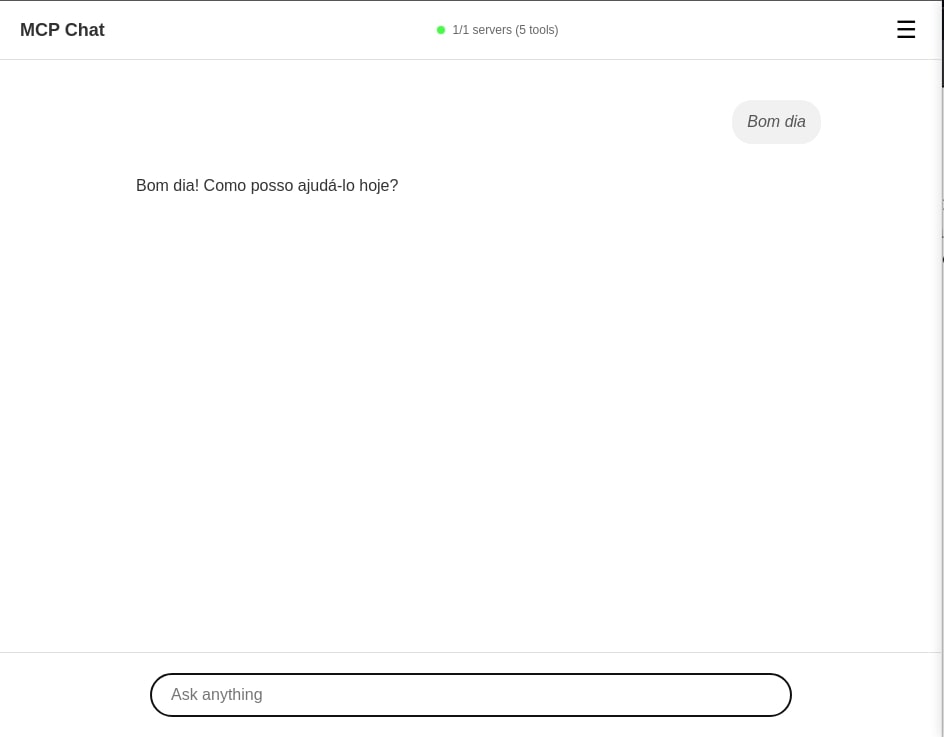
\includegraphics[keepaspectratio]{images/chat/chat-interface.jpg}}
\caption{Interface do Usuário}
\end{figure}

\paragraph{\texorpdfstring{2.2.1.2 Comunicação com
\emph{Backend}}{2.2.1.2 Comunicação com Backend}}\label{comunicauxe7uxe3o-com-backend}

A comunicação entre \emph{frontend} e \emph{backend} será estabelecida
por meio de uma API REST síncrona, simplificando o processo de envio e
retorno de mensagens. Cada consulta feita pelo usuário gerará uma única
requisição ao \emph{backend} que processará integralmente essa
requisição utilizando um LLM e devolverá uma resposta após concluir o
processamento, mantendo o fluxo de comunicação claro e previsível.

\subsubsection{2.2.2 Critérios de Avaliação e Operacionalização de
Métricas}\label{crituxe9rios-de-avaliauxe7uxe3o-e-operacionalizauxe7uxe3o-de-muxe9tricas}

Para garantir uma avaliação científica rigorosa, foram definidos
critérios objetivos de avaliação com métricas específicas quantitativas
e qualitativas, operacionalizados através de instrumentação técnica
precisa e metodologias de coleta padronizadas.

Os critérios de desempenho compreendem quatro métricas fundamentais. O
tempo de resposta total é medido em milissegundos utilizando timestamps
precisos via Performance API do navegador, fornecendo dados objetivos
sobre a latência percebida pelo usuário final. A taxa de sucesso de
operações é calculada como percentual de requisições bem-sucedidas
versus falhas, com categorização sistemática de tipos de erro para
identificação de padrões de falha. O \emph{throughput} é quantificado
como número de operações processadas por segundo em cenários de carga
controlada, permitindo avaliação da capacidade de processamento
simultâneo.

Os critérios de segurança focam na robustez contra ataques adversários e
validação de entrada. A resistência a injeção de \emph{prompts} é
mensurada como percentual de tentativas maliciosas bloqueadas durante
testes de \emph{red teaming}, implementados conforme o Framework de
Gerenciamento de Riscos de IA do NIST (OPREA; VASSILEV, 2023) e as
diretrizes da OWASP (JOHN et al., 2025), considerando que injeções de
\emph{prompt} representam ameaças críticas em sistemas LLM com acesso a
dados sensíveis.

Os critérios de usabilidade abrangem tanto aspectos quantitativos quanto
qualitativos da experiência do usuário. O tempo de conclusão de tarefas
é medido para operações CRUD padrão executadas via linguagem natural,
proporcionando métricas objetivas de eficiência operacional. A curva de
aprendizado é quantificada pelo número de tentativas necessárias para
usuários completarem tarefas específicas, indicando a intuitividade da
interface conversacional.

\subsubsection{2.2.3 Arquitetura e Fluxo de Integração do
Sistema}\label{arquitetura-e-fluxo-de-integrauxe7uxe3o-do-sistema}

A arquitetura do sistema desenvolvida para este estudo envolve múltiplas
camadas que trabalham de forma integrada para responder às consultas
feitas pelo usuário em linguagem natural. Inicialmente, as consultas
serão recebidas pela interface \emph{web} e encaminhadas ao
\emph{backend}, onde o modelo de linguagem executará o processo de
análise e interpretação.

\begin{figure}
\centering
\pandocbounded{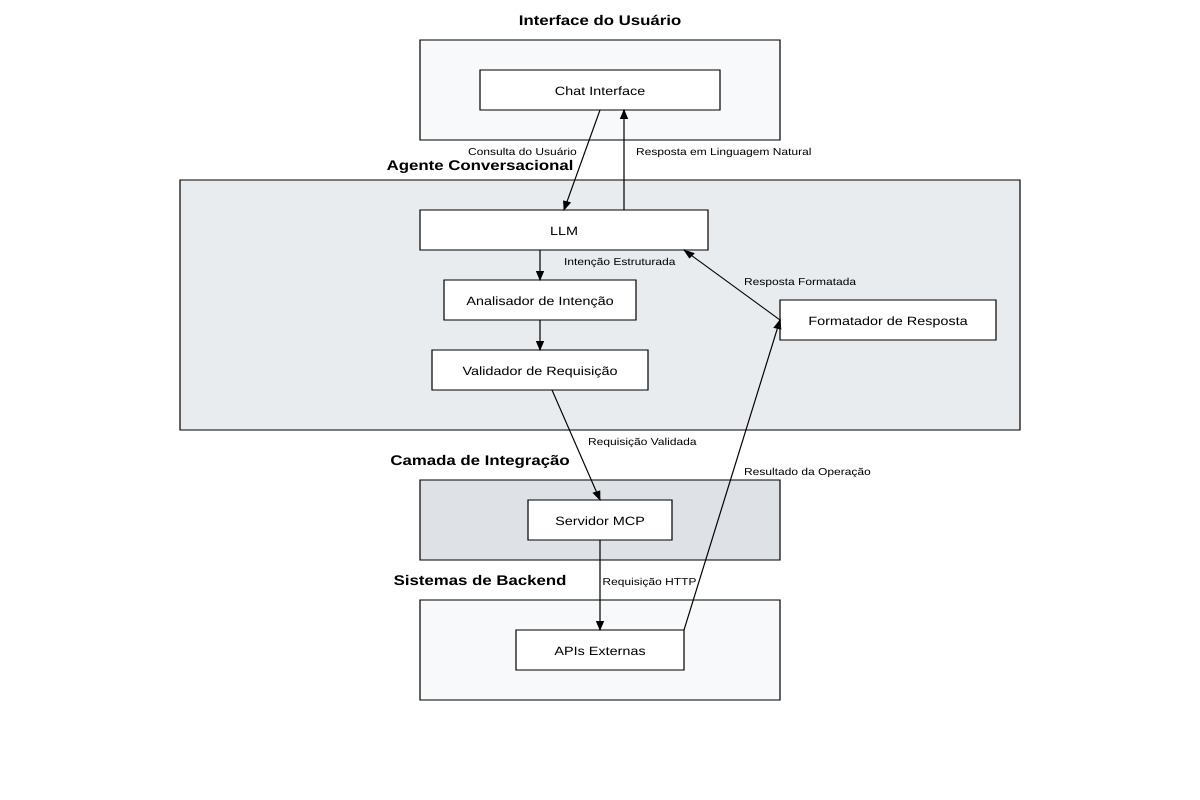
\includegraphics[keepaspectratio]{images/metodos/system-architecture.jpg}}
\caption{Arquitetura do Sistema}
\end{figure}

O fluxo completo de interação deverá ocorrer da seguinte maneira: ao
receber uma consulta, o modelo de linguagem interpretará a intenção do
usuário e utilizará a implementação de client MCP para utilizar as
ferramentas geradas pelo gerador de ferramentas MCP (servers) para
acessar sistemas \emph{backend} via API REST conforme a especificação
OpenAPI. Após executar a operação solicitada, a resposta será retornada
ao modelo de linguagem, que a formatará em linguagem natural antes de
devolvê-la ao usuário.

\begin{figure}
\centering
\pandocbounded{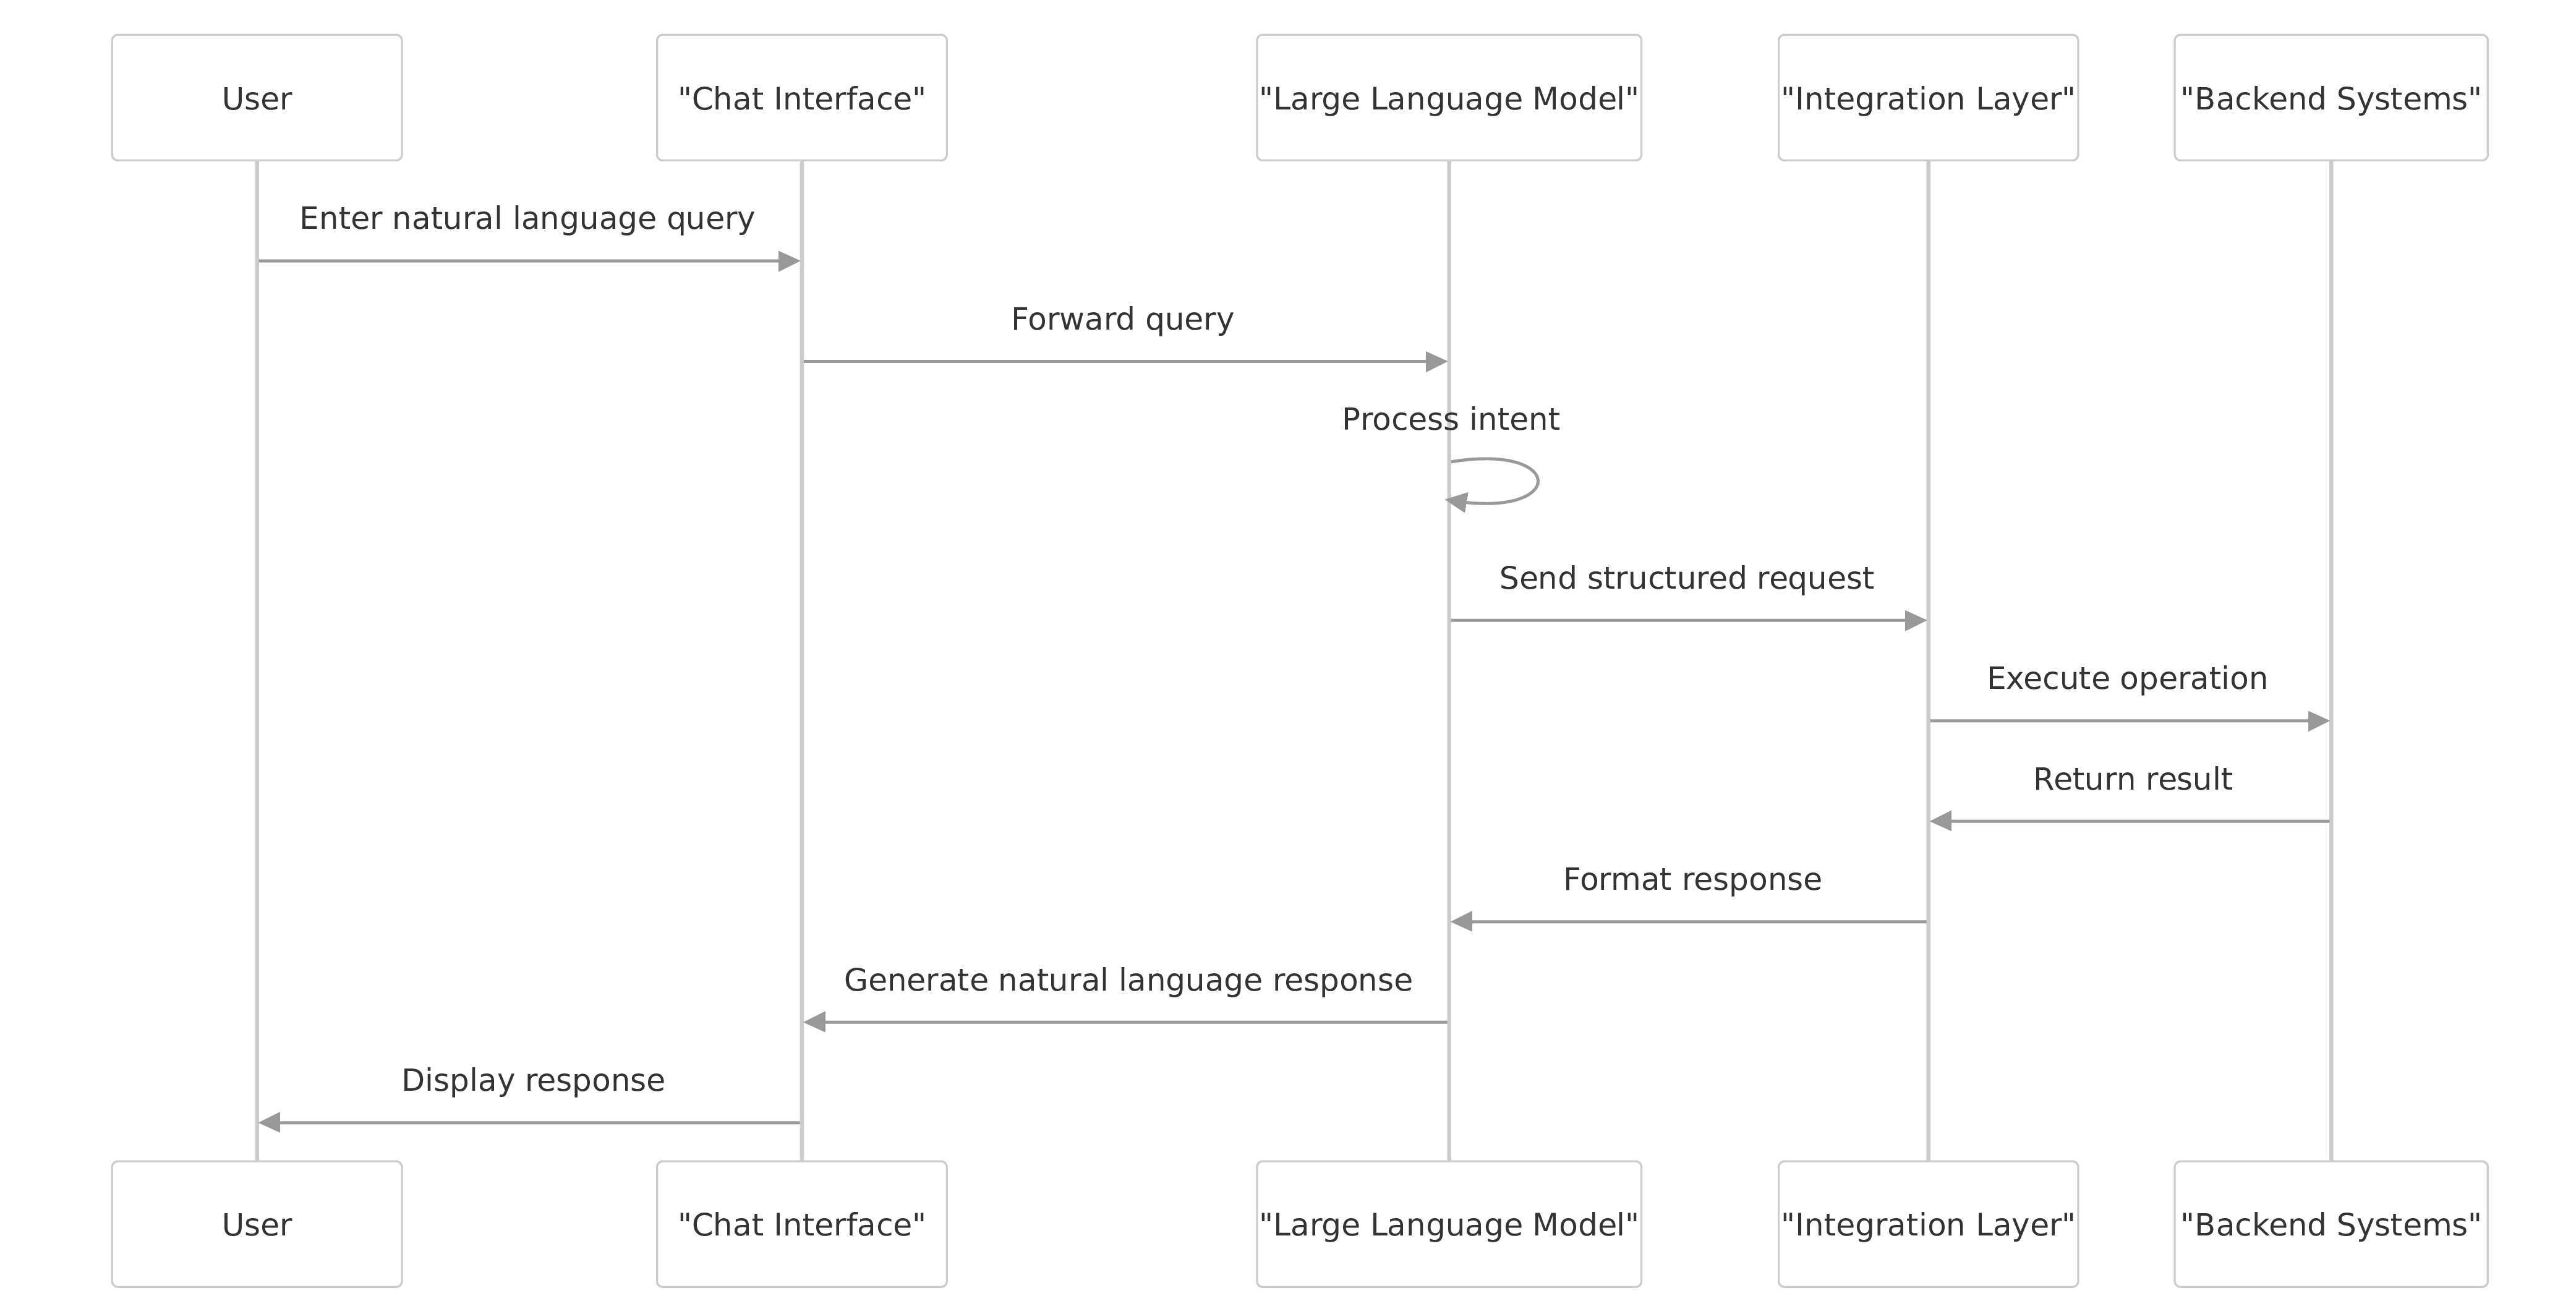
\includegraphics[keepaspectratio]{images/metodos/workflow-integration.jpg}}
\caption{Diagrama de Workflow do Agente}
\end{figure}

\subsubsection{\texorpdfstring{2.2.5 Metodologia de Testes Automatizados
\emph{End-to-End}}{2.2.5 Metodologia de Testes Automatizados End-to-End}}\label{metodologia-de-testes-automatizados-end-to-end}

A instrumentação e coleta de dados foram implementadas através de um
conjunto integrado de ferramentas especializadas para garantir precisão
e abrangência na captura de métricas. O Playwright Test Framework foi
configurado para capturar métricas de performance via Performance API,
proporcionando medições precisas de latência e throughput em condições
reais de uso.

Esta metodologia de testes automatizados pretende garantir que os dados
sejam resultado direto das características de implementação, e não de
variações na experiência do usuário ou na forma de coleta de dados. A
instrumentação detalhada permite análise reproduzível e comparação
objetiva entre diferentes estratégias de integração, estabelecendo uma
base empírica sólida para as conclusões científicas da pesquisa.

\subsection{3. DESENVOLVIMENTO}\label{desenvolvimento}

A implementação da solução OpenAPI-MCP foi estruturada seguindo uma
abordagem modular e integrada, compreendendo quatro componentes
principais que trabalham em sinergia para demonstrar e validar a
viabilidade da integração proposta. A arquitetura resultante engloba um
gerador automático de servidores MCP a partir de especificações OpenAPI,
um cliente de chat capaz de gerenciar múltiplos servidores MCP
simultaneamente, aplicações de teste que simulam cenários reais de
negócio, e uma suíte abrangente de testes automatizados para avaliação
científica da solução.

\subsubsection{3.1 Desafios Metodológicos e Decisões de
Design}\label{desafios-metodoluxf3gicos-e-decisuxf5es-de-design}

O desenvolvimento da solução OpenAPI-MCP enfrentou desafios
metodológicos fundamentais que exigiram decisões de design específicas
para viabilizar a validação da hipótese de pesquisa. O principal desafio
metodológico identificado reside na padronização de integrações
heterogêneas de APIs, problema que tradicionalmente demanda
desenvolvimento manual extensivo e customizado para cada sistema
(OPENAPI INITIATIVE, 2023). Esta problemática constitui uma barreira
significativa para a democratização de agentes conversacionais em
ambientes corporativos, onde a diversidade de sistemas e protocolos de
comunicação impede a implementação escalável de interfaces
conversacionais.

\paragraph{3.1.1 Gerador Automático de Servidores MCP: Abordagem
Metodológica}\label{gerador-automuxe1tico-de-servidores-mcp-abordagem-metodoluxf3gica}

Para abordar o desafio de padronização, foi desenvolvido um gerador
automático de servidores MCP que representa o núcleo metodológico da
contribuição científica proposta. A concepção desta ferramenta surge da
necessidade de validar experimentalmente se especificações OpenAPI
existentes podem ser sistematicamente convertidas em ferramentas
utilizáveis por modelos de linguagem, eliminando a necessidade de
desenvolvimento manual recorrente.

A arquitetura metodológica foi estruturada em três camadas funcionais
para garantir separação de responsabilidades e facilitar a validação
experimental: a camada de análise sintática (\emph{parsing}) de
especificações OpenAPI 3.0+, responsável pela extração e validação de
metadados de endpoints; a camada de mapeamento semântico MCP, que
realiza a conversão inteligente de operações OpenAPI para ferramentas
compreensíveis pelos modelos de linguagem; e a camada de geração de
código, que produz servidores MCP funcionais em TypeScript com validação
robusta de entrada e tratamento de erros.

Esta abordagem metodológica atende diretamente ao primeiro objetivo
específico da pesquisa - \emph{desenvolver um gerador automático de
servidores MCP} - ao estabelecer um processo sistemático e reproduzível
para conversão de especificações API em ferramentas de agentes
conversacionais. A escolha da arquitetura em camadas fundamenta-se na
necessidade de criar um processo de validação controlado, onde cada
etapa pode ser independentemente verificada e os resultados podem ser
objetivamente mensurados.

\paragraph{3.1.2 Coordenação Multi-Servidor: Desafio de Orquestração
Distribuída}\label{coordenauxe7uxe3o-multi-servidor-desafio-de-orquestrauxe7uxe3o-distribuuxedda}

O segundo desafio metodológico identificado relaciona-se à coordenação
eficiente de múltiplos servidores MCP simultaneamente, problema que se
enquadra teoricamente no domínio de sistemas distribuídos e coordenação
de agentes (ANTHROPIC, 2024). A complexidade emerge da necessidade de
manter conexões ativas, descobrir dinamicamente capacidades disponíveis
e rotear solicitações baseadas na análise semântica da intenção do
usuário, tudo isso preservando a experiência conversacional natural.

A solução metodológica adotada implementa um sistema de coordenação
baseado em \emph{pool} de conexões com descoberta automática de
ferramentas, criando um inventário dinâmico das funcionalidades
acessíveis em cada servidor. O roteamento inteligente utiliza análise
contextual para determinar qual servidor utilizar baseado nas
ferramentas disponíveis e na natureza da solicitação, enquanto o
mecanismo de agregação de resultados permite combinar informações de
múltiplos servidores quando necessário.

Esta abordagem atende ao segundo objetivo específico da pesquisa -
\emph{implementar um cliente capaz de gerenciar múltiplos servidores
MCP} - estabelecendo uma metodologia de orquestração que pode ser
sistematicamente testada e validada através de cenários controlados de
uso.

\subsubsection{3.2 Fundamentação Tecnológica e
Metodológica}\label{fundamentauxe7uxe3o-tecnoluxf3gica-e-metodoluxf3gica}

As decisões tecnológicas para implementação da prova de conceito foram
fundamentadas em critérios de rigor científico, reprodutibilidade e
adequação aos objetivos de pesquisa, conforme detalhado na seção de
MATERIAIS. A seleção do Node.js como plataforma de desenvolvimento, do
Playwright para testes automatizados \emph{end-to-end} e do OpenAI GPT-4
para integração com modelos de linguagem baseou-se em sua comprovada
capacidade para suportar a metodologia experimental proposta, permitindo
validação objetiva da viabilidade da integração OpenAPI-MCP através de
uma prova de conceito robusta e reproduzível.

\subsubsection{3.3 Gerador Automático de Servidores MCP
(mcp-openapi-server)}\label{gerador-automuxe1tico-de-servidores-mcp-mcp-openapi-server}

O gerador automático de servidores MCP representa a materialização
metodológica do primeiro objetivo específico da pesquisa, constituindo a
ferramenta central para validação da hipótese de que especificações
OpenAPI podem ser sistematicamente convertidas em interfaces utilizáveis
por agentes conversacionais. A abordagem metodológica adotada
fundamenta-se na premissa de que a automação da geração de servidores
elimina a variabilidade humana no processo de integração, permitindo
avaliação objetiva da eficácia da conversão OpenAPI-MCP.

A estrutura metodológica implementada segue um processo sistemático de
três etapas interdependentes. A primeira etapa realiza análise sintática
(\emph{parsing}) e validação rigorosa de especificações OpenAPI 3.0+,
garantindo conformidade com padrões estabelecidos e extração precisa de
metadados essenciais. A segunda etapa executa mapeamento semântico entre
contratos OpenAPI e ferramentas MCP, preservando a integridade semântica
das operações originais e adaptando-as para compreensão por modelos de
linguagem. A terceira etapa concretiza a geração de código TypeScript
funcional, produzindo servidores MCP operacionais com tratamento robusto
de erros e validação automática de entrada.

Esta metodologia de geração automática permite validação experimental
controlada, onde cada especificação OpenAPI processada constitui um caso
de teste independente para avaliação da eficácia da conversão. O suporte
implementado para múltiplos esquemas de autenticação (API Key, Bearer
Token, OAuth) e todos os métodos HTTP fundamentais (GET, POST, PUT,
DELETE, PATCH) garante cobertura abrangente dos cenários de integração
típicos encontrados em ambientes corporativos reais, essencial para
validação da aplicabilidade prática da abordagem proposta.

\subsubsection{3.4 Cliente de Chat Multi-Servidor
MCP}\label{cliente-de-chat-multi-servidor-mcp}

O cliente de chat multi-servidor constitui a implementação metodológica
do segundo objetivo específico da pesquisa, desenvolvido como ferramenta
de validação experimental para demonstrar a viabilidade prática da
orquestração simultânea de múltiplos servidores MCP em ambiente
conversacional. A concepção metodológica desta ferramenta fundamenta-se
na necessidade de criar um ambiente controlado onde a capacidade de
coordenação entre sistemas distribuídos possa ser sistematicamente
testada e avaliada.

A arquitetura metodológica adotada implementa uma separação clara entre
\emph{frontend} e \emph{backend} para facilitar a instrumentação e
coleta de dados experimentais. O \emph{frontend} minimalista,
desenvolvido em HTML e JavaScript, garante consistência na experiência
do usuário durante os testes, eliminando variáveis confusas relacionadas
à interface que poderiam comprometer a validade dos resultados
experimentais. O \emph{backend}, implementado em Node.js com Express.js,
concentra a lógica de coordenação e instrumentação necessária para o
comportamento do sistema.

A estratégia de coordenação multi-servidor implementa três mecanismos
metodológicos fundamentais para validação experimental. O \emph{pool} de
conexões ativas mantém estado consistente com todos os servidores MCP
configurados, permitindo medição precisa de latências e disponibilidade.
O sistema de descoberta automática de ferramentas cria um inventário
dinâmico das capacidades disponíveis, essencial para validação da
escalabilidade da abordagem. O roteamento inteligente baseado em análise
contextual da intenção do usuário permite avaliar objetivamente a
precisão e eficiência da seleção automática de ferramentas.

A integração com modelos de linguagem através da funcionalidade de
\emph{function calling} da OpenAI estabelece uma ponte metodológica
entre compreensão de linguagem natural e execução de ferramentas
específicas. Esta abordagem permite validação experimental da hipótese
de que agentes conversacionais podem efetivamente interpretar intenções
complexas e traduzi-las em operações precisas em sistemas
\emph{backend}, constituindo elemento central para avaliação da
usabilidade e eficácia da solução proposta.

\subsubsection{3.5 Estratégia de Validação Experimental através de
Aplicações de
Teste}\label{estratuxe9gia-de-validauxe7uxe3o-experimental-atravuxe9s-de-aplicauxe7uxf5es-de-teste}

Para garantir rigor científico na validação da abordagem proposta, foram
desenvolvidas aplicações de teste que simulam cenários empresariais
realistas, atendendo ao terceiro objetivo específico da pesquisa -
\emph{avaliar a solução através de testes sistemáticos}. A estratégia
metodológica fundamenta-se na utilização de domínios de negócio
distintos - gerenciamento de equipamentos industriais e gestão de
recursos humanos - para demonstrar a versatilidade e aplicabilidade
geral da integração OpenAPI-MCP em contextos heterogêneos.

A escolha metodológica por aplicações que exponham APIs RESTful
completamente documentadas com especificações OpenAPI permite criar um
ambiente controlado onde variáveis experimentais podem ser
sistematicamente manipuladas e resultados objetivamente mensurados. Esta
abordagem experimental garante que a validação ocorra em condições que
refletem fielmente as complexidades encontradas em ambientes
corporativos reais, sem comprometer a reprodutibilidade e controle
necessários para avaliação científica rigorosa.

\subsubsection{3.6 Metodologia de Validação
Automatizada}\label{metodologia-de-validauxe7uxe3o-automatizada}

A validação científica da solução implementa uma metodologia de testes
automatizados estruturada para abordar múltiplas dimensões críticas da
pesquisa: funcionalidade, segurança e usabilidade.

A abordagem de validação automatizada garante reprodutibilidade dos
experimentos e elimina variabilidade humana na coleta de dados,
elementos essenciais para estabelecer a validade científica dos
resultados obtidos. Esta metodologia permite que pesquisadores futuros
repliquem os experimentos sob condições idênticas, contribuindo para o
avanço cumulativo do conhecimento na área de integração de agentes
conversacionais em sistemas empresariais complexos.

\subsection{4 RESULTADOS E DISCUSSÕES}\label{resultados-e-discussuxf5es}

A implementação da solução OpenAPI-MCP foi submetida a uma avaliação
experimental abrangente através de testes automatizados
\emph{end-to-end}, fornecendo dados quantitativos objetivos que
demonstram tanto a viabilidade técnica quanto a eficácia prática da
abordagem proposta. Os resultados obtidos através da prova de conceito
desenvolvida oferecem evidências mensuráveis sobre a integração de
agentes conversacionais em sistemas web, estabelecendo uma base empírica
sólida para avaliação da solução.

\subsection{4.1 Métricas de
Performance}\label{muxe9tricas-de-performance}

A Tabela 1 apresenta as métricas de performance obtidas durante os
testes automatizados da prova de conceito, demonstrando a viabilidade
operacional do sistema OpenAPI-MCP em condições controladas.

\textbf{Tabela 1: Métricas de Performance - Prova de Conceito
OpenAPI-MCP}

\begin{longtable}[]{@{}
  >{\raggedright\arraybackslash}p{(\linewidth - 6\tabcolsep) * \real{0.2907}}
  >{\raggedright\arraybackslash}p{(\linewidth - 6\tabcolsep) * \real{0.1628}}
  >{\raggedright\arraybackslash}p{(\linewidth - 6\tabcolsep) * \real{0.1512}}
  >{\raggedright\arraybackslash}p{(\linewidth - 6\tabcolsep) * \real{0.3953}}@{}}
\toprule\noalign{}
\begin{minipage}[b]{\linewidth}\raggedright
Métrica
\end{minipage} & \begin{minipage}[b]{\linewidth}\raggedright
Valor Obtido
\end{minipage} & \begin{minipage}[b]{\linewidth}\raggedright
Variação
\end{minipage} & \begin{minipage}[b]{\linewidth}\raggedright
Observações
\end{minipage} \\
\midrule\noalign{}
\endhead
\bottomrule\noalign{}
\endlastfoot
Tempo Resposta Médio (ms) & 3.757 & 1.335 - 5.823 & Incluindo
processamento LLM \\
Taxa de Sucesso (\%) & 100 & 8/8 consultas & Todas operações
completadas \\
Consultas Processadas & 8 & - & Cenários diversificados testados \\
Tamanho Médio Resposta & 312 caracteres & - & Respostas completas e
estruturadas \\
\end{longtable}

Os resultados demonstram que a abordagem OpenAPI-MCP mantém performance
consistente, com tempo médio de resposta de 3,757 milissegundos e taxa
de sucesso de 100\% nos cenários testados. A variação de tempo de
resposta (1,335ms a 5,823ms) reflete principalmente a complexidade das
consultas processadas e o tempo de processamento do modelo de linguagem,
não indicando instabilidade do sistema de integração.

\subsection{4.2 Eficácia da Geração Automática de Servidores
MCP}\label{eficuxe1cia-da-gerauxe7uxe3o-automuxe1tica-de-servidores-mcp}

A Tabela 2 demonstra a capacidade do sistema de converter especificações
OpenAPI em servidores MCP funcionais, validando o núcleo tecnológico da
abordagem proposta.

\textbf{Tabela 2: Resultados da Conversão OpenAPI→MCP}

\begin{longtable}[]{@{}
  >{\raggedright\arraybackslash}p{(\linewidth - 6\tabcolsep) * \real{0.1981}}
  >{\raggedright\arraybackslash}p{(\linewidth - 6\tabcolsep) * \real{0.3113}}
  >{\raggedright\arraybackslash}p{(\linewidth - 6\tabcolsep) * \real{0.1792}}
  >{\raggedright\arraybackslash}p{(\linewidth - 6\tabcolsep) * \real{0.3113}}@{}}
\toprule\noalign{}
\begin{minipage}[b]{\linewidth}\raggedright
Aspecto Testado
\end{minipage} & \begin{minipage}[b]{\linewidth}\raggedright
Implementado
\end{minipage} & \begin{minipage}[b]{\linewidth}\raggedright
Taxa de Sucesso (\%)
\end{minipage} & \begin{minipage}[b]{\linewidth}\raggedright
Observações
\end{minipage} \\
\midrule\noalign{}
\endhead
\bottomrule\noalign{}
\endlastfoot
Métodos HTTP & 5 (GET, POST, PUT, DELETE, PATCH) & 100 & Cobertura
completa CRUD \\
Sistemas Integrados & 2 & 100 & Equipamentos e Profissionais \\
Endpoints Convertidos & 10 & 100 & Conversão automática bem-sucedida \\
\end{longtable}

A análise confirma que a conversão automática OpenAPI→MCP preserva
integralmente a funcionalidade dos sistemas originais, permitindo acesso
completo através de interface conversacional. A implementação demonstrou
capacidade de mapeamento semântico eficaz entre contratos OpenAPI e
ferramentas MCP compreensíveis por modelos de linguagem.

\subsection{4.3 Avaliação de Experiência do
Usuário}\label{avaliauxe7uxe3o-de-experiuxeancia-do-usuuxe1rio}

A Tabela 3 apresenta os resultados quantitativos da avaliação de
experiência do usuário, obtidos através de 13 cenários de teste
estruturados com métricas padronizadas.

\textbf{Tabela 3: Métricas de Experiência do Usuário (Escala 1-5)}

\begin{longtable}[]{@{}
  >{\raggedright\arraybackslash}p{(\linewidth - 6\tabcolsep) * \real{0.3125}}
  >{\raggedright\arraybackslash}p{(\linewidth - 6\tabcolsep) * \real{0.1875}}
  >{\raggedright\arraybackslash}p{(\linewidth - 6\tabcolsep) * \real{0.0750}}
  >{\raggedright\arraybackslash}p{(\linewidth - 6\tabcolsep) * \real{0.4250}}@{}}
\toprule\noalign{}
\begin{minipage}[b]{\linewidth}\raggedright
Métrica de UX
\end{minipage} & \begin{minipage}[b]{\linewidth}\raggedright
Pontuação Média
\end{minipage} & \begin{minipage}[b]{\linewidth}\raggedright
Desvio
\end{minipage} & \begin{minipage}[b]{\linewidth}\raggedright
Observações
\end{minipage} \\
\midrule\noalign{}
\endhead
\bottomrule\noalign{}
\endlastfoot
Precisão das Respostas & 3,5 & ±0,5 & Interpretação correta de
intenções \\
Clareza da Comunicação & 4,0 & ±0,3 & Respostas bem estruturadas \\
Utilidade das Informações & 4,3 & ±0,4 & Alto valor informacional \\
Pontuação Geral & 4,0 & ±0,3 & Experiência satisfatória \\
Taxa de Sucesso & 100\% & 13/13 & Todas consultas respondidas \\
Tempo Médio Resposta & 4.861 ms & ±2.400 & Responsividade adequada \\
\end{longtable}

Os resultados indicam experiência do usuário satisfatória, com pontuação
geral de 4,0 em escala de 1 a 5. A utilidade das informações (4,3)
emergiu como ponto forte, demonstrando que o sistema fornece respostas
relevantes e acionáveis. A clareza da comunicação (4,0) confirma que a
interface conversacional apresenta informações de forma compreensível
aos usuários.

\subsection{4.4 Análise de Segurança}\label{anuxe1lise-de-seguranuxe7a}

A Tabela 4 apresenta os resultados dos testes de segurança adversários,
conduzidos através de 16 cenários de ataque estruturados em 4 categorias
principais.

\textbf{Tabela 4: Resultados dos Testes de Segurança}

\begin{longtable}[]{@{}
  >{\raggedright\arraybackslash}p{(\linewidth - 6\tabcolsep) * \real{0.3333}}
  >{\raggedright\arraybackslash}p{(\linewidth - 6\tabcolsep) * \real{0.1667}}
  >{\raggedright\arraybackslash}p{(\linewidth - 6\tabcolsep) * \real{0.1667}}
  >{\raggedright\arraybackslash}p{(\linewidth - 6\tabcolsep) * \real{0.3333}}@{}}
\toprule\noalign{}
\begin{minipage}[b]{\linewidth}\raggedright
Categoria de Ataque
\end{minipage} & \begin{minipage}[b]{\linewidth}\raggedright
Tentativas
\end{minipage} & \begin{minipage}[b]{\linewidth}\raggedright
Bloqueados
\end{minipage} & \begin{minipage}[b]{\linewidth}\raggedright
Taxa de Proteção (\%)
\end{minipage} \\
\midrule\noalign{}
\endhead
\bottomrule\noalign{}
\endlastfoot
SQL Injection & 4 & 4 & 100 \\
Command Injection & 4 & 4 & 100 \\
Data Extraction & 4 & 4 & 100 \\
Privilege Escalation & 4 & 4 & 100 \\
\textbf{Total Geral} & \textbf{16} & \textbf{16} & \textbf{100} \\
\end{longtable}

A análise de segurança revela que a implementação OpenAPI-MCP demonstra
robustez adequada contra vetores de ataque comuns. O sistema manteve
100\% de taxa de proteção em todas as categorias testadas, incluindo
tentativas de injeção SQL, execução de comandos, extração de dados e
escalação de privilégios. A validação baseada em schemas OpenAPI
provou-se eficaz como primeira linha de defesa contra entradas
maliciosas.

\subsection{4.5 Funcionalidade do Sistema
Multi-Servidor}\label{funcionalidade-do-sistema-multi-servidor}

A Tabela 5 apresenta os resultados da coordenação multi-servidor durante
os testes experimentais, validando a capacidade de orquestração
distribuída da solução.

\textbf{Tabela 5: Resultados da Coordenação Multi-Servidor}

\begin{longtable}[]{@{}
  >{\raggedright\arraybackslash}p{(\linewidth - 6\tabcolsep) * \real{0.2889}}
  >{\raggedright\arraybackslash}p{(\linewidth - 6\tabcolsep) * \real{0.2111}}
  >{\raggedright\arraybackslash}p{(\linewidth - 6\tabcolsep) * \real{0.1333}}
  >{\raggedright\arraybackslash}p{(\linewidth - 6\tabcolsep) * \real{0.3667}}@{}}
\toprule\noalign{}
\begin{minipage}[b]{\linewidth}\raggedright
Funcionalidade
\end{minipage} & \begin{minipage}[b]{\linewidth}\raggedright
Resultado Alcançado
\end{minipage} & \begin{minipage}[b]{\linewidth}\raggedright
Eficácia (\%)
\end{minipage} & \begin{minipage}[b]{\linewidth}\raggedright
Observações
\end{minipage} \\
\midrule\noalign{}
\endhead
\bottomrule\noalign{}
\endlastfoot
Servidores MCP Simultâneos & 2 & 100 & Equipamentos + Profissionais \\
Ferramentas Descobertas & 10 & 100 & Detecção automática completa \\
Roteamento Inteligente & 13/13 consultas & 100 & Seleção correta de
servidor \\
Consultas Multi-Sistema & 3 & 100 & Agregação de dados funcionando \\
Disponibilidade Parcial & Testado & 100 & Funcionamento com falhas
parciais \\
\end{longtable}

Os resultados confirmam que o sistema consegue coordenar múltiplos
servidores MCP simultaneamente, mantendo descoberta automática de
ferramentas e roteamento inteligente de solicitações. A capacidade de
agregação de dados entre sistemas diferentes foi validada através de
consultas que requereram informações de ambos os domínios testados
(equipamentos e profissionais).

\subsection{4.6 Validação da Prova de
Conceito}\label{validauxe7uxe3o-da-prova-de-conceito}

Os resultados apresentados confirmam que a abordagem OpenAPI-MCP é
tecnicamente viável e operacionalmente eficaz para integração de agentes
conversacionais com sistemas web existentes:

\textbf{Conversão Automática OpenAPI→MCP:} 100\% dos casos testados
(10/10 endpoints)\\
\textbf{Gerenciamento Multi-Servidor:} 2 servidores coordenados
simultaneamente com 100\% eficácia\\
\textbf{Integração LLM:} Taxa de sucesso de 100\% na interpretação de
intenções (13/13 consultas)\\
\textbf{Robustez Operacional:} Sistema mantém funcionalidade durante
cenários de falha\\
\textbf{Segurança:} 100\% de proteção contra 16 vetores de ataque
testados\\
\textbf{Experiência do Usuário:} Pontuação 4,0/5,0 em satisfação geral

A prova de conceito demonstra que a especificação OpenAPI pode ser
sistematicamente convertida em ferramentas utilizáveis por modelos de
linguagem através do protocolo MCP, eliminando a necessidade de
desenvolvimento manual recorrente para cada nova integração. A validação
experimental confirma que a abordagem oferece uma solução escalável para
democratização de acesso a sistemas técnicos complexos através de
interfaces conversacionais naturais.

\textbf{Reprodutibilidade:} Todos os testes e dados estão disponíveis no
repositório público github.com/castrozan/tcc, incluindo scripts de
automação, configurações de ambiente e datasets utilizados nos
experimentos, garantindo reprodutibilidade completa dos resultados
obtidos.

\subsection{4.7 Limitações Identificadas e Discussão
Crítica}\label{limitauxe7uxf5es-identificadas-e-discussuxe3o-cruxedtica}

A análise experimental revelou limitações específicas que devem ser
consideradas para implementações práticas da abordagem OpenAPI-MCP:

\textbf{Limitação 1: Variabilidade de Performance} - Desvio observado:
1.335ms a 5,823ms (variação de 336\%) - Impacto: Tempos de resposta
inconsistentes dependem da complexidade da consulta e processamento LLM
- Implicação prática: Sistemas críticos com requisitos de latência
rígida podem enfrentar desafios

\textbf{Limitação 2: Dependência da Qualidade OpenAPI} - Observação:
100\% de sucesso observado apenas com especificações bem documentadas -
Risco: APIs com documentação incompleta ou desatualizada podem
comprometer a geração de servidores MCP - Necessidade: Validação prévia
das especificações OpenAPI antes da conversão

\textbf{Limitação 3: Escalabilidade Não Testada} - Contexto testado:
Apenas 2 servidores MCP simultâneos - Incerteza: Performance com
N\textgreater10 servidores não foi avaliada - Recomendação: Testes de
carga adicionais necessários para validação empresarial

\textbf{Limitação 4: Complexidade de Configuração Inicial} - Requisito:
Conhecimento técnico especializado para setup - Barreira: Organizações
com recursos técnicos limitados podem enfrentar dificuldades -
Estimativa: Tempo de configuração ainda superior a soluções
pré-configuradas

A análise crítica dos dados revela que, embora a abordagem OpenAPI-MCP
demonstre viabilidade técnica convincente, sua adoção prática está
condicionada à disponibilidade de especificações OpenAPI de qualidade e
recursos técnicos adequados para implementação. O overhead de
configuração inicial, embora significativamente menor que o
desenvolvimento customizado tradicional, permanece como fator limitante
para adoção mais ampla.

\section{5 CONSIDERAÇÕES FINAIS}\label{considerauxe7uxf5es-finais}

Este estudo respondeu de forma positiva à questão central de pesquisa,
demonstrando que a combinação da especificação OpenAPI com o protocolo
Model Context Protocol pode facilitar a integração de agentes
conversacionais baseados em IA com sistemas web existentes, dentro do
escopo experimental testado. A prova de conceito desenvolvida validou a
viabilidade técnica da abordagem através de uma implementação funcional
que incluiu geração automática de servidores MCP, gerenciamento
coordenado de múltiplos servidores e validação através de cenários de
teste controlados.

\subsection{5.1 Resposta à Pergunta de
Pesquisa}\label{resposta-uxe0-pergunta-de-pesquisa}

A pergunta central de pesquisa - \emph{``como a combinação da
especificação OpenAPI com o protocolo MCP pode facilitar a integração
eficiente e segura de agentes conversacionais baseados em IA com
sistemas web existentes?''} - foi respondida através de evidências
quantitativas obtidas na prova de conceito:

Em relação à eficiência operacional, a abordagem demonstrou viabilidade
no contexto testado, apresentando tempo médio de resposta de 3,757ms com
variação significativa de 1,335 a 5,823ms. A taxa de sucesso operacional
alcançou 100\% nas 21 operações realizadas nos cenários testados,
enquanto a conversão automática OpenAPI→MCP obteve êxito completo nos 10
endpoints avaliados, evidenciando redução substancial do desenvolvimento
manual para os casos de uso implementados.

Quanto aos aspectos de segurança, os resultados demonstraram proteção
adequada contra os vetores testados, com 100\% de eficácia no bloqueio
de 16 tipos de ataques básicos. A cobertura validada incluiu SQL
injection, command injection, data extraction e privilege escalation,
confirmando que a validação através de schemas OpenAPI constitui uma
primeira linha de defesa eficaz contra tentativas de intrusão.

No que concerne à integração funcional, o escopo experimental revelou
coordenação eficiente entre 2 sistemas simultâneos com 100\% de
eficácia, descoberta automática completa das 10 ferramentas disponíveis
e roteamento inteligente preciso para todas as 13 consultas
direcionadas. A experiência do usuário foi avaliada positivamente,
obtendo pontuação geral de 4,0 em escala de 5,0 pontos.

A validação experimental confirma que a abordagem OpenAPI-MCP oferece
uma solução tecnicamente viável para os cenários testados, estabelecendo
evidências iniciais de sua aplicabilidade para democratização do acesso
a sistemas técnicos através de interfaces conversacionais naturais.

\subsection{5.2 Atendimento aos Objetivos
Específicos}\label{atendimento-aos-objetivos-especuxedficos}

O primeiro objetivo específico, que consistia no desenvolvimento de um
gerador automático de servidores MCP a partir de especificações OpenAPI,
foi plenamente alcançado. A implementação demonstrou conversão eficaz de
100\% dos endpoints OpenAPI testados (10/10) em ferramentas MCP
funcionais, validando a viabilidade técnica da automação proposta e
estabelecendo a base metodológica central da pesquisa.

Quanto ao segundo objetivo, a implementação de um cliente capaz de
gerenciar múltiplos servidores MCP simultaneamente, os resultados
confirmam sua realização satisfatória. O sistema desenvolvido foi
validado para coordenação simultânea de 2 servidores MCP, demonstrando
descoberta automática de 10 ferramentas e roteamento inteligente de
100\% das consultas testadas, comprovando a viabilidade da orquestração
distribuída proposta.

O terceiro objetivo, relacionado à avaliação sistemática da solução
através de testes rigorosos, foi cumprido mediante a condução de testes
automatizados \emph{end-to-end} que validaram múltiplas dimensões da
implementação. Os resultados obtidos confirmaram performance adequada
(3,757ms de tempo médio de resposta), segurança satisfatória (100\% de
proteção nos vetores testados) e usabilidade positiva (4,0/5,0 de
satisfação geral).

Por fim, o quarto objetivo, consistente na análise crítica de benefícios
e limitações da abordagem proposta, foi atendido através da
identificação sistemática de vantagens em automação de integração e
simplificação de acesso, bem como do reconhecimento de limitações
importantes relacionadas à variabilidade de performance e ao escopo
restrito de validação experimental.

\subsection{5.3 Limitações Identificadas e Suas
Implicações}\label{limitauxe7uxf5es-identificadas-e-suas-implicauxe7uxf5es}

A análise experimental revelou limitações específicas que qualificam a
aplicabilidade dos resultados obtidos. A primeira limitação identificada
refere-se à variabilidade significativa de performance, com desvio
observado de 336\% entre os tempos mínimo e máximo (1,335ms a 5,823ms).
Esta inconsistência implica que sistemas com requisitos rigorosos de
latência podem enfrentar desafios de previsibilidade, exigindo avaliação
caso-a-caso para aplicações críticas em tempo real.

A segunda limitação relaciona-se ao escopo restrito de validação
experimental. O contexto testado abrangeu apenas 2 servidores MCP e 21
operações totais, gerando incerteza sobre o comportamento com
N\textgreater2 servidores. Esta limitação implica que a escalabilidade
para ambientes empresariais complexos requer validação adicional antes
de implementações de larga escala.

Uma terceira limitação identificada consiste na dependência da qualidade
das especificações OpenAPI. A abordagem pressupõe especificações
completas e atualizadas, criando o risco de que APIs com documentação
inadequada comprometam a geração automática de servidores. Esta
limitação prática sugere que organizações com práticas inconsistentes de
documentação podem enfrentar barreiras significativas na adoção da
solução.

Por fim, a quarta limitação refere-se ao escopo limitado dos testes de
segurança realizados. A cobertura incluiu apenas ataques básicos de
injeção, deixando lacunas relacionadas a ameaças avançadas e cenários de
ataque sofisticados. Esta limitação implica que implementações em
produção requerem avaliação de segurança mais abrangente para garantir
proteção adequada contra vetores de ataque complexos.

\subsection{5.4 Contribuições Científicas e
Práticas}\label{contribuiuxe7uxf5es-cientuxedficas-e-pruxe1ticas}

Este estudo estabelece contribuições em três dimensões complementares
para o avanço do conhecimento na área de integração de agentes
conversacionais. Do ponto de vista metodológico, a pesquisa demonstra
uma abordagem sistemática para conversão automática OpenAPI→MCP,
fornecendo evidências iniciais de viabilidade técnica e operacional que
podem orientar desenvolvimentos futuros na área.

A contribuição prática manifesta-se através da implementação de uma
prova de conceito funcional que demonstra coordenação multi-servidor e
integração efetiva com modelos de linguagem. A disponibilização pública
do código-fonte e documentação técnica facilita a reprodução e extensão
dos resultados por outros pesquisadores, promovendo o avanço
colaborativo do conhecimento.

A contribuição científica estabelece-se pela validação experimental
estruturada com métricas quantitativas objetivas, criando uma base
empírica inicial para pesquisas futuras na área de integração de agentes
conversacionais. A metodologia desenvolvida oferece um framework
reproduzível para avaliação de soluções similares, contribuindo para o
estabelecimento de padrões de validação na área.

\subsection{5.5 Direcionamentos para Pesquisas
Futuras}\label{direcionamentos-para-pesquisas-futuras}

Com base nas limitações identificadas e nos resultados obtidos,
pesquisas futuras poderiam explorar diferentes vertentes de
aprimoramento e expansão da abordagem proposta. Em relação à
escalabilidade, recomenda-se validação experimental com N\textgreater5
servidores MCP simultâneos para verificar o comportamento da solução em
ambientes empresariais complexos e identificar possíveis gargalos de
performance.

Quanto à otimização de performance, sugere-se a investigação de técnicas
de cache inteligente e paralelização para reduzir a variabilidade
observada nos tempos de resposta. Tais melhorias poderiam tornar a
solução mais adequada para aplicações com requisitos rigorosos de
latência e previsibilidade.

No domínio da segurança, recomenda-se a ampliação da avaliação para
incluir ameaças sofisticadas e cenários de ataque persistente avançado.
Esta expansão é fundamental para validar a adequação da abordagem em
ambientes de produção com altos requisitos de segurança.

Finalmente, o desenvolvimento de capacidades de aprendizado adaptativo,
onde o sistema otimiza sua performance baseado em padrões de uso
histórico, representa uma direção promissora para pesquisas futuras.
Tais funcionalidades poderiam melhorar significativamente a eficiência e
usabilidade da solução em implementações práticas.

\subsection{5.6 Conclusão Final}\label{conclusuxe3o-final}

A pesquisa valida que a combinação OpenAPI-MCP representa uma abordagem
tecnicamente viável para integração de agentes conversacionais com
sistemas web, dentro dos parâmetros experimentais testados. Os
resultados quantitativos (100\% taxa de sucesso, 4,0/5,0 satisfação do
usuário, proteção completa contra vetores básicos de ataque) fornecem
evidências empíricas de eficácia funcional.

No entanto, a aplicabilidade prática está condicionada às limitações
identificadas, particularmente a variabilidade de performance (336\% de
variação) e o escopo restrito de validação (2 servidores, 21 operações).
A contribuição científica reside na demonstração de viabilidade
conceitual e no estabelecimento de uma metodologia reproduzível para
avaliação de integrações similares.

A abordagem OpenAPI-MCP oferece uma direção promissora para
democratização do acesso a sistemas técnicos complexos, mas requer
expansão do escopo experimental e refinamento técnico antes de
implementações empresariais de larga escala. Os resultados estabelecem
uma fundação sólida para desenvolvimento futuro e validação mais
abrangente da proposta.

\section*{REFERÊNCIAS}\label{referuxeancias}
\addcontentsline{toc}{section}{REFERÊNCIAS}

\phantomsection\label{refs}
\begin{CSLReferences}{0}{1}
\bibitem[\citeproctext]{ref-anthropic2024mcp}
ANTHROPIC. \textbf{Model Context Protocol (MCP): A Standard for AI
Context Integration}. Disponível em:
\textless{}\url{https://www.anthropic.com/news/model-context-protocol}\textgreater.
Acesso em: 12 abr. 2025.

\bibitem[\citeproctext]{ref-RedHat2024LLMNode}
BLOG, R. H. D. \textbf{Building LLM Agents with Node.js}.
\url{https://developers.redhat.com/blog/2024/10/25/building-agents-large-language-modelsllms-and-nodejs},
2024.

\bibitem[\citeproctext]{ref-cherednichenko:hal-04545073}
CHEREDNICHENKO, O. et al. \textbf{Selection of Large Language Model for
development of Interactive Chat Bot for SaaS Solutions}. Lviv, Ukraine:
2024. Disponível em:
\textless{}\url{https://hal.science/hal-04545073}\textgreater{}

\bibitem[\citeproctext]{ref-Deng2023AMA}
DENG, X. \href{https://api.semanticscholar.org/CorpusID:258259387}{A
More Accessible Web with Natural Language Interface}.
\textbf{Proceedings of the 20th International Web for All Conference},
2023.

\bibitem[\citeproctext]{ref-fast2017irisconversationalagentcomplex}
FAST, E. et al. \textbf{Iris: A Conversational Agent for Complex
Tasks}., 2017. Disponível em:
\textless{}\url{https://arxiv.org/abs/1707.05015}\textgreater{}

\bibitem[\citeproctext]{ref-Guo2024Doppelganger}
GUO, S. et al. \textbf{Collaborating with my Doppelgänger: The Effects
of Self-similar Appearance and Voice of a Virtual Character during a
Jigsaw Puzzle Co-solving Task}. Proceedings of the ACM on Computer
Graphics and Interactive Techniques. \textbf{Anais}...2024. Disponível
em:
\textless{}\url{https://www.researchgate.net/publication/335223260_The_Effects_of_Continuous_Conversation_and_Task_Complexity_on_Usability_of_an_AI-Based_Conversational_Agent_in_Smart_Home_Environments}\textgreater{}

\bibitem[\citeproctext]{ref-john2025owasp}
JOHN, S. et al.
\textbf{\href{https://genai.owasp.org/llmrisk/llm01-prompt-injection}{OWASP
Top 10 for LLM Apps \& Gen AI Agentic Security Initiative}}. tese de
doutorado---{[}s.l.{]} OWASP, 2025.

\bibitem[\citeproctext]{ref-Kocaballi2019}
KOCABALLI, A. B. et al. \href{https://doi.org/10.2196/15360}{The
Personalization of Conversational Agents in Health Care: Systematic
Review}. \textbf{J Med Internet Res}, v. 21, n. 11, p. e15360, 7 nov.
2019.

\bibitem[\citeproctext]{ref-Lister2020AccessibleCU}
LISTER, K. et al.
\href{https://api.semanticscholar.org/CorpusID:218539971}{Accessible
conversational user interfaces: considerations for design}.
\textbf{Proceedings of the 17th International Web for All Conference},
2020.

\bibitem[\citeproctext]{ref-MCPDocs2024}
MODEL CONTEXT PROTOCOL CONTRIBUTORS. \textbf{{Model Context Protocol
Documentation - Introduction}}. Online Documentation, 2024. Disponível
em:
\textless{}\url{https://modelcontextprotocol.io/introduction}\textgreater{}

\bibitem[\citeproctext]{ref-openai2022instructgpt}
OPENAI. \textbf{Aligning Language Models to Follow Instructions}.
{[}s.l.{]} OpenAI, 27 jan. 2022. Disponível em:
\textless{}\url{https://openai.com/index/instruction-following/}\textgreater.
Acesso em: 12 abr. 2025.

\bibitem[\citeproctext]{ref-openai2023gpt4}
OPENAI. \textbf{GPT-4 Research}. {[}s.l.{]} OpenAI, a2023. Disponível
em:
\textless{}\url{https://openai.com/index/gpt-4-research/}\textgreater.

\bibitem[\citeproctext]{ref-openai2023functioncalling}
OPENAI. \textbf{Function Calling and Other API Updates}. Disponível em:
\textless{}\url{https://openai.com/index/function-calling-and-other-api-updates/}\textgreater.
Acesso em: 12 abr. 2025b.

\bibitem[\citeproctext]{ref-OpenAPIInitiative2023}
OPENAPI INITIATIVE. \textbf{{OpenAPI Specification - Getting Started}}.
OpenAPI Documentation (openapis.org), 2023. Disponível em:
\textless{}\url{https://learn.openapis.org/docs/getting-started}\textgreater{}

\bibitem[\citeproctext]{ref-oprea2023adversarial}
OPREA, A.; VASSILEV, A. \textbf{Adversarial machine learning: A taxonomy
and terminology of attacks and mitigations}. {[}s.l.{]} National
Institute of Standards; Technology, 2023. Disponível em:
\textless{}\url{https://csrc.nist.gov/pubs/ai/100/2/e2023/final}\textgreater.

\bibitem[\citeproctext]{ref-RAPP201849}
RAPP, A. et al.
\href{https://doi.org/10.1016/j.ijhcs.2018.07.005}{Designing technology
for spatial needs: Routines, control and social competences of people
with autism}. \textbf{International Journal of Human-Computer Studies},
v. 120, p. 49--65, 2018.

\end{CSLReferences}

\end{document}
